\documentclass[tikz,border=10pt]{standalone}
\usepackage{tikz}
\usetikzlibrary{positioning, shapes, arrows, fit}

\begin{document}

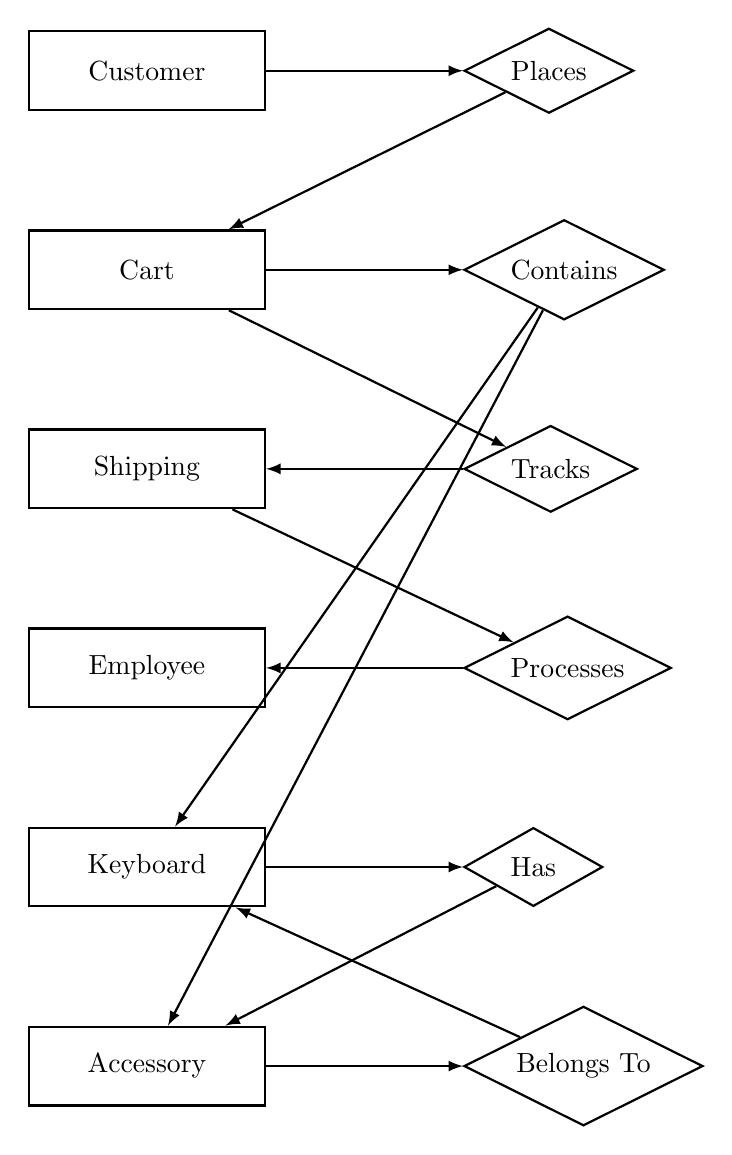
\begin{tikzpicture}[
    entity/.style={rectangle, draw=black, thick, minimum width=3cm, minimum height=1cm, align=center},
    relation/.style={diamond, draw=black, thick, aspect=2, minimum width=1cm, minimum height=1cm, align=center},
    attribute/.style={ellipse, draw=black, thick, minimum width=1.5cm, minimum height=0.7cm, align=center},
    link/.style={draw, thick, -latex}
]

% Entities
\node[entity] (Customer) {Customer};
\node[entity, below=1.5cm of Customer] (Cart) {Cart};
\node[entity, below=1.5cm of Cart] (Shipping) {Shipping};
\node[entity, below=1.5cm of Shipping] (Employee) {Employee};
\node[entity, below=1.5cm of Employee] (Keyboard) {Keyboard};
\node[entity, below=1.5cm of Keyboard] (Accessory) {Accessory};

% Relationships
\node[relation, right=2.5cm of Customer] (Places) {Places};
\node[relation, right=2.5cm of Cart] (Contains) {Contains};
\node[relation, right=2.5cm of Shipping] (Tracks) {Tracks};
\node[relation, right=2.5cm of Employee] (Processes) {Processes};
\node[relation, right=2.5cm of Keyboard] (Has) {Has};
\node[relation, right=2.5cm of Accessory] (BelongsTo) {Belongs To};

% Connections
\draw[link] (Customer) -- (Places);
\draw[link] (Places) -- (Cart);
\draw[link] (Cart) -- (Contains);
\draw[link] (Contains) -- (Keyboard);
\draw[link] (Contains) -- (Accessory);
\draw[link] (Cart) -- (Tracks);
\draw[link] (Tracks) -- (Shipping);
\draw[link] (Shipping) -- (Processes);
\draw[link] (Processes) -- (Employee);
\draw[link] (Keyboard) -- (Has);
\draw[link] (Has) -- (Accessory);
\draw[link] (Accessory) -- (BelongsTo);
\draw[link] (BelongsTo) -- (Keyboard);

\end{tikzpicture}

\end{document}

